\documentclass[11pt]{amsart}
\usepackage{amsmath,amsfonts,amsthm,amssymb, amsaddr}
\usepackage{graphicx}


\title{Lorentz Transformations}

\author{Joe Bentley}

\date{\today}

\begin{document}

\maketitle

\newpage


\section{Galilean Tranformations}

Galilean transformations describe a set of transformations between two inertial frames in space. For frame $\Sigma'$ moving at velocity $v$ in the positive x-direction, away from a stationary frame $\Sigma$, we have the following for each coordinate in space and time,

\begin{align*}
x' &= x - vt \\
y' &= y \\
z' &= z \\
t' &= t \\
\end{align*}

y', z', and t' are all constant in time as the moving frame $\Sigma'$ is not changing in any of those directions, and time is considered universal across all reference frames. By differentiating the x coordinate with respect to time we can find an expression for the velocity $u'_x$ measured by $\Sigma'$ of a body moving at velocity $u_x$ in $\Sigma$. Of course we expect to see the velocity added to the frame's velocity. For example, if we are stationary and we throw a ball at 40mph, we
expect an observer moving towards the ball at 10mph to see the ball going 30mph. We see that this is indeed the case,

\begin{align}
\label{eq:galilean}
u'_x = u_x - v
\end{align}

\section{Lorentz Transformations}

Special relativity tells us that we would measure the same velocity for light in any reference frame, no matter our relative velocities. This means we may need a new set of transformations to describe transformations between these inertial frames of reference as our case of velocities adding as in eq.~\ref{eq:galilean}.

Again we will consider two frames, a stationary frame $\Sigma$ and a frame $\Sigma'$ moving at velocity $v$ in the $x$-direction. First we will consider the most general case of transformations. We will use constant before each term in our transformations, and find the value of these constants. Here is our general form,

\begin{align*}
x' &= Ax - Bct \text{  eq(a)} \\
y' &= y \\
z' &= z \\
ct' &= Ex - Dct \text{  eq(b)}
\end{align*}

Again we can say that there is no relative motion in the $y'$ and $z'$ as there is no velocity in those directions, but we will not make the assumption that time is universal in all frames of reference just yet, as that may be wrong due to special relativity. We use $ct$ in time so that everything has dimensions of length, and also we will use only linear terms or else the laws of physics would differ at different points in space, which we assume isn't true.

\section{Point of View from $\Sigma$}

Firstly we consider the view from $\Sigma$. $\Sigma$ sees the origin of $\Sigma'$ moving away at a velocity $v$. At this point we have $x = vt'$ and $x' = 0$ (as it is at the origin).

\begin{align*}
\text{in eq(a) we have  } \to 0 = Avt + Bct \implies B = -\frac{Av}{c}
\end{align*}

Thus we have,

\begin{align}
\label{eq:B}
B = -\frac{Av}{c}
\end{align}

\section{Point of View from $\Sigma'$}

We now consider that $\Sigma'$ sees the origin at $\Sigma$ moving away (in the negative x-direction). Now we have $x = -vt'$ and $x = 0$ (at the origin).

\begin{align*}
\text{in eq(a)  } \to -vt' &= 0 + Bct = -Avt \text{  from eq.~\ref{eq:B}} \\
\text{in eq(b)  } \to ct' &= 0 + Dct \implies t' = Dt \\
\end{align*}

Therefore we now have,

\begin{align*}
t' = Dt \to -vDt = -Avt \to D = A
\end{align*}

We now have another relation,

\begin{align}
\label{eq:D}
D = A
\end{align}

\section{$\Sigma$ Fires Beam of Light}

We now take the case where $\Sigma$ fires a beam of light along the x-axis at t = 0. The location given in $\Sigma$ and $\Sigma'$ is $x = ct$ and $x' = ct'$ respectively, because c is the same in all frames of reference.

\begin{align*}
\text{using eq(a):  } x' &= ct' = Ax + Bct = Act + Bct \\
\text{from eq~\ref{eq:B}  } ct' &= A\left(ct - vt\right) \\
\text{also, using eq(b)  } ct' &= Ect + Dct = Ect + Act \text{  (by eq~\ref{eq:D})} \\
\to A\left(ct - vt\right) &= Act - Avt = Ect + Act
\end{align*}

We therefore have that,

\begin{align}
\label{eq:E}
E = -\frac{Av}{c} = B
\end{align}

\section{Light Pulse emitted in y-direction}

Now we take the case as a light pulse is emitted in the y-direction in $\Sigma$ at $t = 0$. In $\Sigma'$ the pulse has both an x and y-component, as $\Sigma'$ is moving in the x-direction relative to $\Sigma$ and is thus moving relative to the light. We know however that the velocity is $c$ in both $\Sigma$ and $\Sigma'$ due to special relativity.

So, in $\Sigma$ we have $x = 0$ and $y = ct$, in $\Sigma'$ we have $x'^2 + y'^2 = c^2 t'^2$ (from Pythagoras' theorem).

In the x-direction we have,

\begin{align*}
\text{in eq(a):  } x'^2 &= \left(Ax + Bct\right)^2 \\
                        &= A^2\left(0 - vt\right)^2 \text{  using eq.~\ref{eq:B}} \\
                        &= A^2 v^2 t^2
\end{align*}

and in the y-direction we have,

\begin{align*}
y'^2 &= y^2 = c^2 t^2 \\
c^2 t'^2 &= \left(Ex + Dct\right)^2 = \left(0 + Act\right)^2 \text{  using eq.~\ref{eq:D}} \\
         &= A^2 c^2 t^2
\end{align*}

Therefore, from $x'^2 + y'^2 = c^2 t'^2$, and by substituting in $x'^2$ and $y'^2$, we have,

\begin{align*}
A^2 v^2 t^2 + c^2 t^2 &= A^2 c^2 t^2
\end{align*}

and then dividing through by $c^2$ and $t^2$,

\begin{align*}
A^2 \frac{v^2}{c^2} + 1 &= A^2 \\
1 &= A^2\left(1 - \frac{v^2}{c^2}\right)
\end{align*}

We thus arrive at our important result,

\begin{align}
\label{eq:gamma}
A = \frac{1}{\sqrt{1 - \frac{v^2}{c^2}}} = \gamma
\end{align}

and,

\begin{align*}
B = -\gamma \frac{v}{c}, D = \gamma, E = -\gamma \frac{v}{c}
\end{align*}

\section{Lorentz Transformations}

Now, by substituting back in all we now know, we arrive at the Lorentz transformations,

\begin{align*}
x' &= \gamma\left[x - vt\right] \\
y' &= y \\
z' &= z \\
ct' &= \gamma\left[ct - \frac{v}{c} x\right]
\end{align*}

One important result in this is the observation that space and time are clearly linked, that is, the spatial transformation includes time, and the temporal transformation includes space. This is the essence of space-time.


\section{Velocity Transformations}

By differentiating the x and t transformations and applying the chain rule, we can find expressions for the velocity, although this will not be shown here as it is quite easy,

\begin{align*}
u_x = \frac{u'_x + v}{1 + \frac{v u'_x}{c^2}}
\end{align*}

\section{Spacetime}

In this section we will define a useful concept known as the space-time interval, which will allow us to easily assess causality connections between events. First we will consider a flash of light in a frame $\Sigma'$ moving relative to a stationary frame $\Sigma$. An observer, $O'$ in the $\Sigma'$ frame will see the flash of light move at a speed $v' = c$. We can express the distance travelled by this light in some time $\Delta t'$ as,

\begin{align}
  \label{eq:spacetime1}
  \Delta r'^2 = c^2 \Delta t'^2
\end{align}

An observer $O$ in $\Sigma$ will also see the flash of light moving at velocity $v = c$,

\begin{align}
  \label{eq:spacetime2}
  \Delta r^2 = c^2 \Delta t^2
\end{align}

For both eq.~\ref{eq:spacetime1} and eq.~\ref{eq:spacetime2} we can see that both can be equated to a constant, zero, and can be equated,

\begin{align*}
  c^2 \Delta t^2 - \Delta r^2 = c^2 \Delta t'^2 - \Delta r'^2
\end{align*}

From this we can define a space-time interval, giving us an interval between two places in spacetime.

\begin{align*}
  \Delta s^2 = c^2 \Delta t^2 - \Delta r^2
\end{align*}

where $\Delta t$ is the difference in time between two events, and $\Delta r$ is the distance between the two points. $\Delta s^2$ is invariant under Lorentz transformation, that is, $c^2 \Delta t^2 - \Delta r^2 = c^2 \Delta t'^2 - \Delta r'^2$. This means that space and time are linked and completely connected, so in general we use a 4-vector to represent spacetime (a 4-vector has a time component as well as spatial components).

How can we interpret our space-time interval $\Delta s^2$? In the case where $\Delta s^2 > 0$ then this is called a "timelikeinterval". In this case the two events can reach each other without going faster than the speed of light, so the events are said to be causally conneted. Here time flows, and at a rate such that the proper time is $\Delta \tau = \left(c^2 \Delta t^2 - \Delta r^2\right)^{\frac{1}{2}}$. Next we will look at the $\Delta s^2 = 0$ which is called a "lightlike"
interval. In this interval no time flows; an observer going at the speed of light would not perceive any time to pass. This interval is such that the proper time $\Delta \tau = 0$. Lastly there is the case where $\Delta s^2 < 0$ called a "spacelike" interval. Here no signal can pass between, as the signal would have to travel faster than the speed of light to be able to do so. This interval is not in the future or past cone of the lightcone diagram, so there is no causal connection.

\section{Momentum in Special Relativity}

We can see that our classical equation for momentum, $\mathbf{p} = m\mathbf{v}$ will not work under the conditions that we need in special relativity. Firstly, if we have a large momentum then we can have a velocity greater than the speed of light; it seems unnatural to put an upper limit on momentum like this. Secondly, it doesn't allow massless particles like photons to have momentum, which we know they do. Also it does not conserve momentum in all reference frames due to velocity transformations. To find a relativistic momentum equation we will consider a glancing collision between two particles.

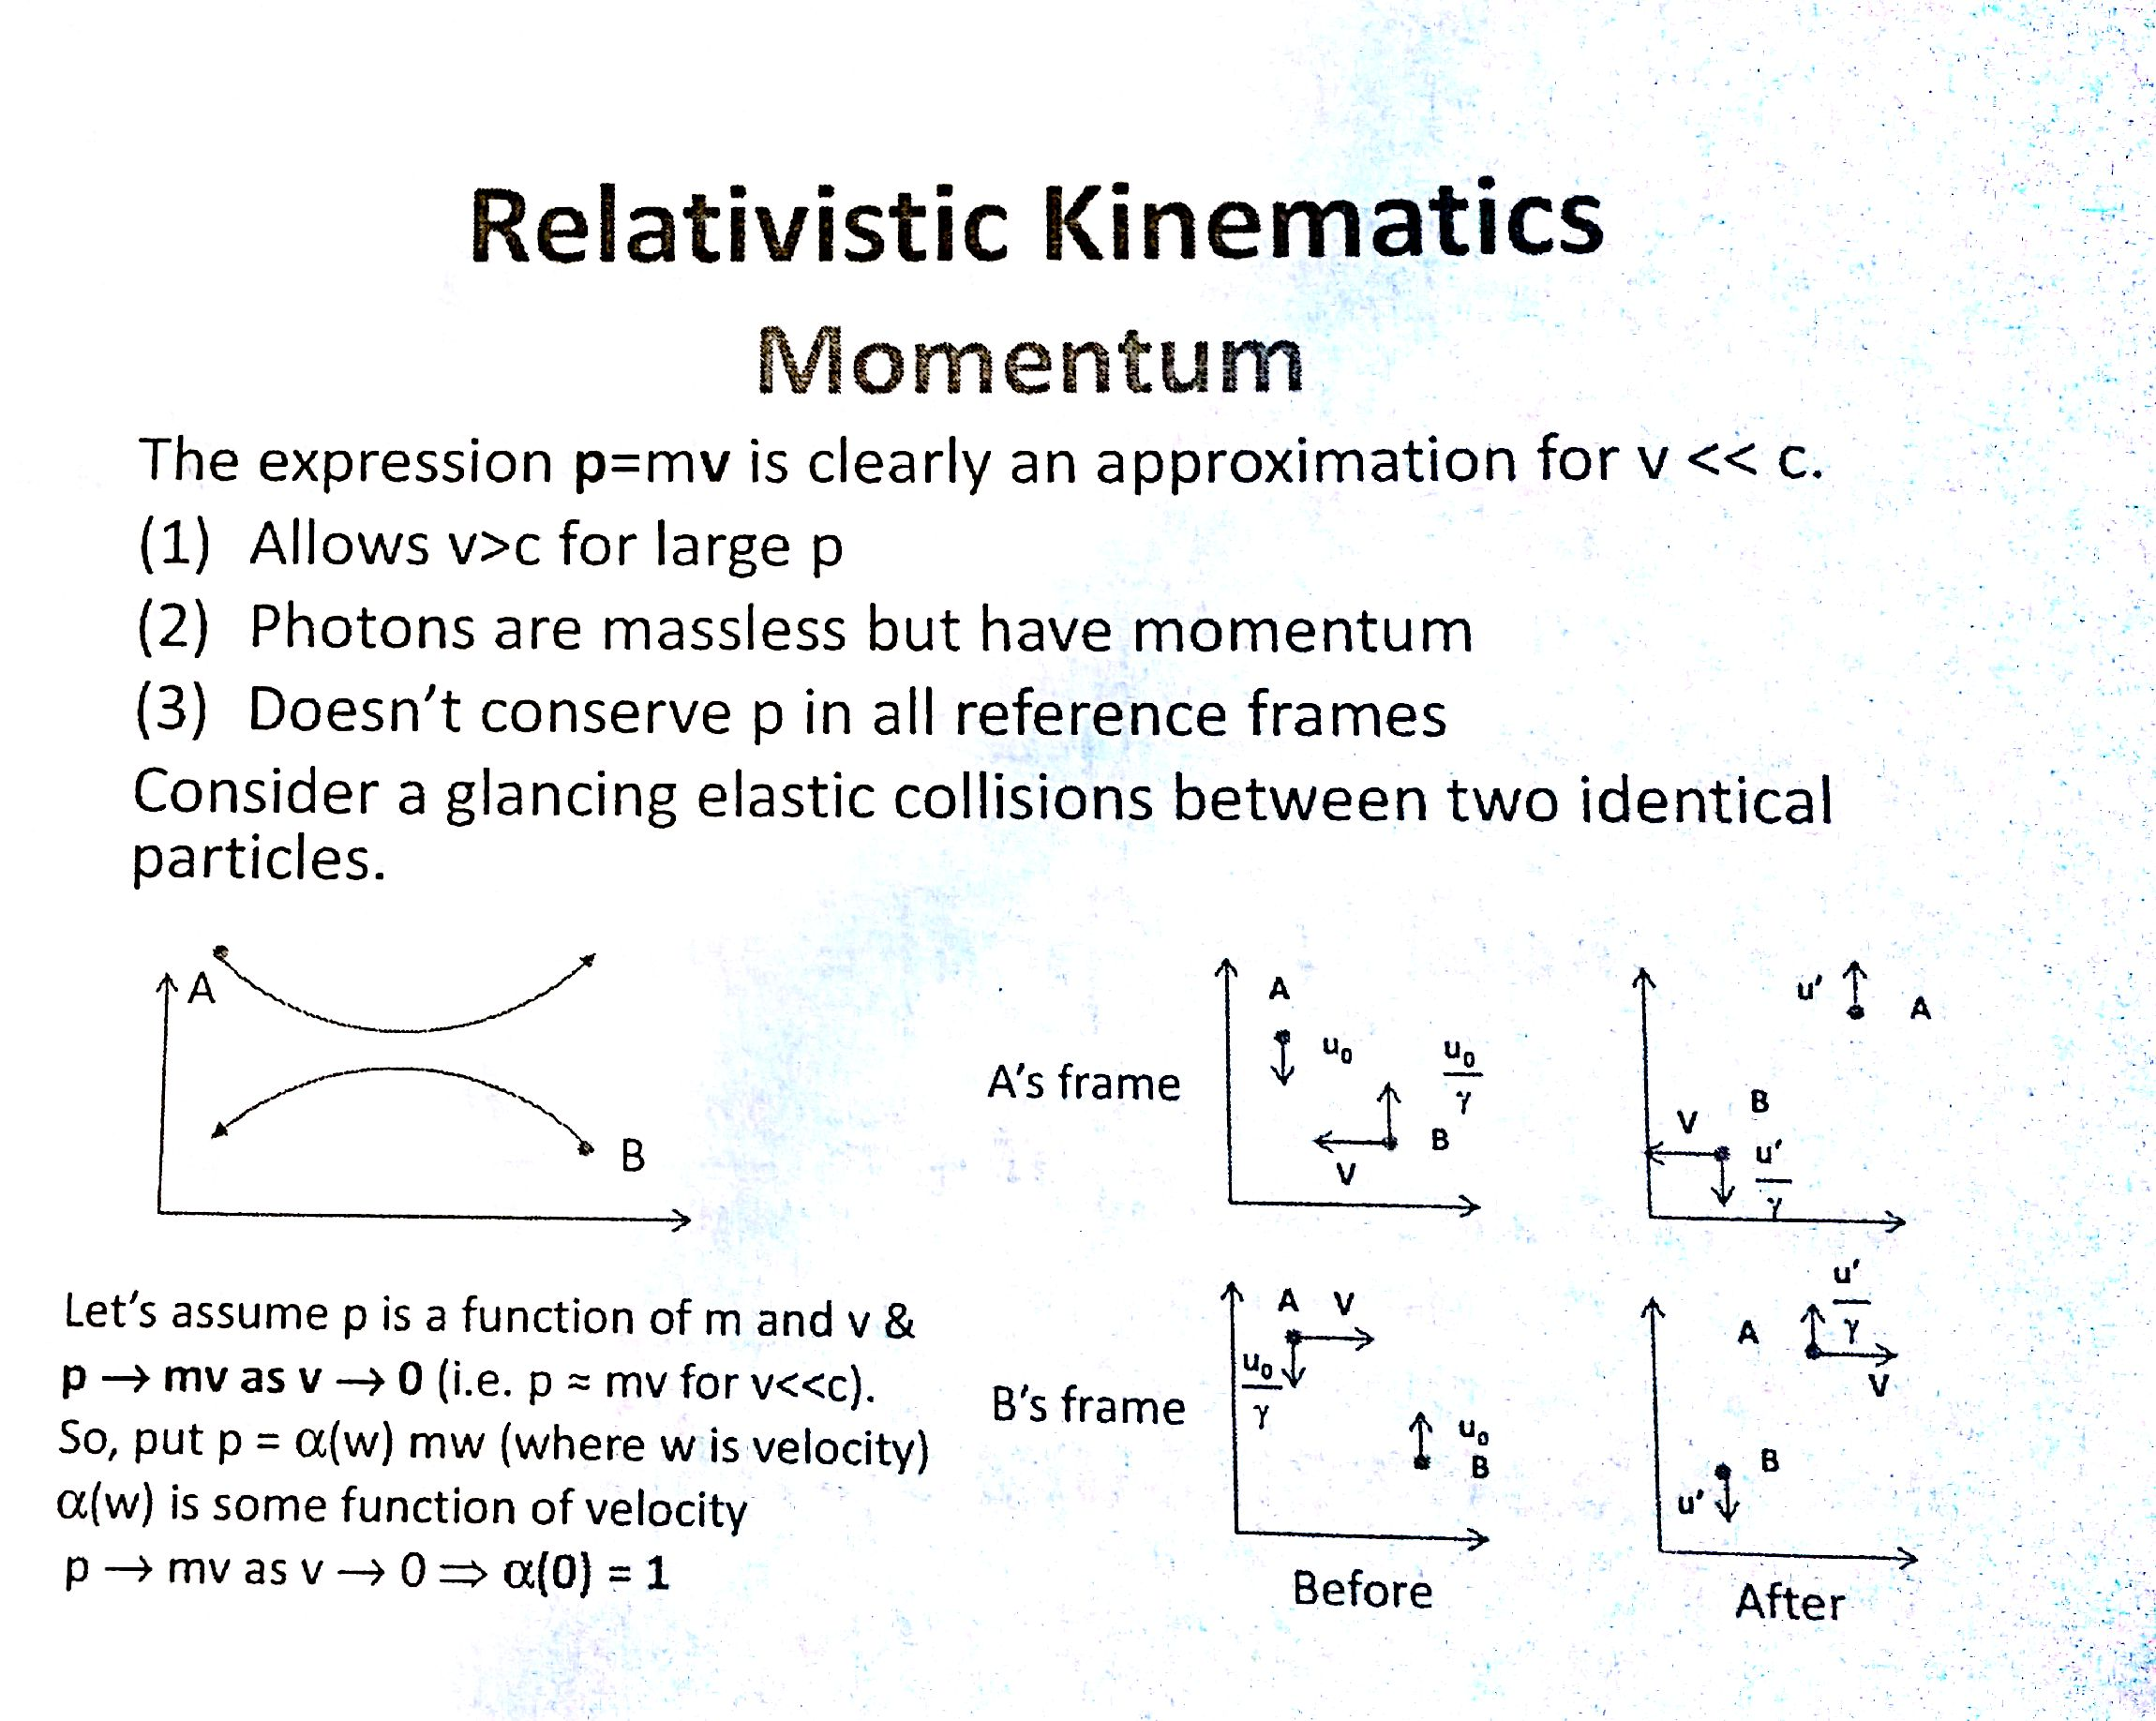
\includegraphics[scale=0.15]{frames}

To formulate an idea of what this might look like, first we will assume that $\mathbf{p}$ must be a function of $m$ and $\mathbf{v}$, and that $\mathbf{p} \to m\mathbf{v}$ as $\mathbf{v} \to 0$. So we will postulate a function of the following form,

\begin{align*}
  \mathbf{p} = \alpha(w) m \mathbf{w}
\end{align*}

where $\alpha(w)$ is some function of the velocity. We use $w$ as we have used both $v$ and $u$ in our diagram. Since $\mathbf{p} \to m\mathbf{v}$ as $\mathbf{v} \to 0$, this means that $\alpha(0) = 1$.

First we will look from A's frame of reference. We can see that B's speed before the collision is,

\begin{align*}
  w &= {\left(v^2 + \frac{u_0^2}{\gamma^2}\right)}^{\frac{1}{2}}
\end{align*}

and B's speed after the collision,

\begin{align*}
  w' &= {\left(v^2 + \frac{u'^2}{\gamma^2}\right)}^{\frac{1}{2}}
\end{align*}

By applying conservation of momentum in the x-direction (just of particle B, as A has no x-component),

\begin{align*}
  m\alpha(w)v &= m\alpha(w')v \\
  \implies \alpha(w) &= \alpha(w') \\
  \implies w &= w' \implies u_0 = u'
\end{align*}

therefore we see that the speed of B doesn't change during the collision. By applying conservation of momentum in the y-direction, now involving both particles. This time we won't write the factors of mass $m$ and we will use that $u_0 = u'$,

\begin{align*}
  -\alpha(u_0) u_0 + \alpha(w)\frac{u_0}{\gamma} &= \alpha(u_0)u_0 - \alpha(w)\frac{u_0}{\gamma} \\
  \alpha(w)\frac{u_0}{\gamma} &= \alpha(u_0) u_0 \\
  \implies \frac{\alpha(w)}{\gamma} &= \alpha(u_0)
\end{align*}

In the limit as $u_0 \to 0$,

\begin{align*}
  \alpha(v) &= \gamma \alpha(0) \\
  \implies \alpha(v) &= \gamma
\end{align*}

where $\gamma = \frac{1}{\sqrt{1-\frac{v^2}{c^2}}}$, the Lorentz factor. Now we have our relativistic equation of momentum,

\begin{align*}
  \mathbf{p} = \gamma m \mathbf{v}
\end{align*}

\end{document}
